\documentclass[11pt,a4paper,twoside,final]{book}
%
\usepackage{ngerman}            %Neue Rechtschreibung
\usepackage{graphicx}           %Graphiken einbinden
%\usepackage[normalsize]{subfigure} %Teilbilder in Bildern mit Querverweis
\usepackage{fontenc}            %Verwenden von \"{o} \"{a} \"{u} {\ss}
\usepackage[utf8]{inputenc}   %Verwenden von ä ö ü ß
\usepackage{fancyhdr}           %Kopf-und Fusszeilen
\usepackage{theorem}			%S�tze, Beispiele und dergleichen
\usepackage{amsmath}			%Setzen von Gleichungen und Formeln
\usepackage{amssymb}			%Mathematische Symbole
\usepackage{bibgerm}			%Deutsches Literaturverzeichnis bei Verwendung von bibtex
\usepackage{longtable}			%Lange Tabellen
\usepackage{booktabs}
\usepackage{helvet}				%Wird f�r die serifenlosen Schriften auf der Titelseite ben�tigt
\usepackage[right]{eurosym}		%Das Eurosymbol
\usepackage{pdflscape}			%Drehen einzelner Seiten ins Querformat
\usepackage{siunitx}			%Setzen von Einheiten
\usepackage{multirow}
\usepackage{caption}
\usepackage{array}
\usepackage{subcaption}
\usepackage{svg}
\usepackage{tikz}				%Ein umfangreiches Paket f�r Graphiken: Nur f�r Fans
\usepackage{algorithm}
\usepackage{algorithmic}
\usepackage{txfonts}
\usepackage{float}
\usepackage{pythonhighlight}
\usepackage{listings}
\usepackage{tikz-uml}


\usetikzlibrary{positioning}
\usetikzlibrary{calc}
\usetikzlibrary{shapes.geometric}
\usetikzlibrary{shapes.arrows}
\usetikzlibrary{decorations}
\usetikzlibrary{decorations.pathmorphing}
\usetikzlibrary{decorations.text}
\usetikzlibrary{decorations.markings}
\usetikzlibrary{backgrounds}
\usetikzlibrary{intersections}
\usetikzlibrary{matrix,chains,positioning,decorations.pathreplacing,arrows}
\graphicspath{{Bilder/}{Bilder/plots/}{Bilder/infer_images/}}

\usepackage[european]{circuitikz}	%Ein Paket zum Zeichnen von Schaltungen

\usepackage{pgfplots}				%Erstellen von Plots

\usepackage[a4paper,
			textwidth = 16.5cm,
			textheight = 25cm,
			inner = 2.5cm]{geometry}
		
		
\usepackage[pdftex,
			colorlinks,
			linkcolor = black,
			citecolor = black]{hyperref}	%Verlinkungen im pdf-Dokument


%
%	Einstellung der Kopf- und Fu�zeilen
%
\pagestyle{fancyplain}
\renewcommand{\chaptermark}[1]{\markboth{#1}{}}
 \renewcommand{\sectionmark}[1]{\markright{\thesection\ #1}}
 \lhead[\fancyplain{}{\sl\thepage}]{\fancyplain{}{\sl\rightmark}}
 \rhead[\fancyplain{}{\sl\leftmark}]{\fancyplain{}{\sl\thepage}}
 \lfoot{}
 \cfoot{}
 \rfoot{}

\setlength{\parindent}{0cm}

%--------------------------------------------------------------------
%
\renewcommand\maketitle{
\begin{titlepage}

\thispagestyle{empty}
%
\begin{tabular}[t]{lp{0.25\textwidth}r}
%
\includegraphics[width = 0.25\textwidth]{./Bilder/Logo_HSRT_TEC_RGB.png}
%
&&\includegraphics[width = 0.4\textwidth]{./Bilder/Logo_HSRT_Schwarz.jpg}
%
\end{tabular}
%

\renewcommand{\baselinestretch}{1.2}

\vspace{2cm}

\begin{center}

\sf\huge{Hochschule Reutlingen}\\
\sf\Large{Reutlingen University}\\

\vspace{2cm}

\sf\Large{-- Studiengang Mechatronik Bachelor --}\\
%
\vspace{0.5cm}

\sf\Large{Bachelor--Thesis}

\vspace{2cm}

{\sf\huge{Entwicklung eines autonomen Systems zur Bilderkennung 
mithilfe Neuronaler Netze auf dedizierter Hardware}}\\

\end{center}

\vspace{3cm}

%
\sf{
Manuel Barkey\\
Pestalozzistraße 29\\
72762 Reutlingen\\
\ \\
Matrikelnummer : 762537

}

\vspace{2cm}

\begin{tabular}{lp{0.5cm}l}
%
Betreuer:				&&Eberhard Binder		\\
Zweitbetreuer:			&&Christian Höfert		\\
Abgabedatum:			&&TT.MM.JJJJ
%
\end{tabular}

\renewcommand{\baselinestretch}{1}
%

\vfill
%

\includegraphics[width = \textwidth]{./Bilder/Silhouette_HSRT_045K.jpg}
%
\newpage
\ 
\thispagestyle{empty}
%
\end{titlepage}}

\theoremstyle{plain}
\theorembodyfont{\itshape}\theoremheaderfont{\bf}
%
%
\newtheorem{defi}{Definition}[chapter]
\newtheorem{beisp}{Beispiel}[chapter]
\newtheorem{regel}{Regel}[chapter]
%
\newenvironment{bsp}{\begin{beisp} }{\end{beisp}}%

%\setcounter{tocdepth}{1}

\newcounter{uebung}
\setcounter{uebung}{1}

		
\title{Abschlussarbeit--Titel}

%--------------------------------------------------------------------

\begin{document}


\maketitle

\setcounter{page}{1}
\setcounter{tocdepth}{1}

\tableofcontents

\thispagestyle{empty}

\chapter{Einleitung}\label{kap:einleitung}

Wildkameras kommen in der Jagt oder zu biologischen 
Forschungszwecken zum Einsatz.
Da das Aufnehmen der Bilder automatisch über einen 
Bewegungsmelder erfolgt, kann es unter Umständen zu 
einer großen Menge an unwichtigen Daten kommen.
Diese benötigen Speicherplatz auf dem Gerät, 
oder, bei automatischem Senden, Datenvolumen 
für die Mobile Netzwerkverbindung und bringen ausserdem einen 
großen Auswertungsaufwand mit sich.

Ein System, welches genau erkennt, um welche Tiere es
sich bei den gemachten Aufnahmen handelt, kann wesentlich 
effizienter und gezielter für eine bestimmte Anwendung 
eingesetzt werden.
Beispielsweise zur Überwachung des eigenen Gartens vor 
Füchsen, oder zum Aufspüren von Wölfen und Bären 
in bestimmten Waldgebieten.
Auch der Artbestand seltener oder aussterbender 
Tierarten könnte so leichter erfasst werden.

Für die Umsetzung einer solchen Bilderkennungsaufgabe 
werden Deep Learning Algorithmen verwendet, welche ein
Teilgebiet der künstlichen Intelligenz sind.
Bei den verwendeten Modellen handelt es sich in der Bilderkennung
meist um sogenannte Convolutional Neural Networks (CNNs).

Durch die Fortschritte, die in diesem Bereich in
den letzten jahren gemacht wurden, sowie durch 
die Verfügbarkeit leistungsfähiger und zugleich
kostengünstiger Hardware, ist die realisierung
einer solchen Anwendung auch für den Privatgebrauch
und ohne Verwendung eines Großrechners möglich geworden.


Ziel der vorliegenden Arbeit war es, ein autonomes Kamerasystem 
zu entwickeln, welches mithilfe von Deep Learning Algorithmen, 
verschiedene Wildtierarten erkennen und klassifizieren kann.
Dieses soll auf einem Raspberry Pi 4 laufen und 
Bilder von erkannten Tieren automatisch an den Nutzer 
senden.
Die Inferenz der Neuronalen Netze wird dabei
auf dem KI Beschleuniger Neural Compute Stick 2
von Intel ausgeführt werden. Durch verwendung einer 
infrarotfähigen Kamera soll die Erkennung des 
Systems auch bei Nacht stattfinden können.

Damit gliedert sich die Arbeit zunächst in ein
Grundlagen Kapitel, welches die funktionsweise 
von künstlichen Neuronalen Netzen für die
Bilderkennung behandelt.
Anschließend wrd es um die Umsetzung und Auswertung des 
Trainings geeigneter Deep Learning Modelle gehen.

Der letzte Teil beschreibt de Entwicklung der Anwendung, 
in welcher die Inferenz eines fertig trainiertes Modell, 
für den Neural Compute Stick, implementiert wird.
\section[\thesection \  Grundlagen]{Grundlagen}\label{sec:grundlagen}



\subsection[\thesection .\thesubsection \ 
Machine Learning]{Machine Learning}\label{subsec:ml}


\begin{frame}{Machine Learning}
        Erkennung von Zusammenhängen in großen Datenmengen,\\ohne explizite Programmierung darauf.
        \begin{itemize}
            \item \textit{Supervised Learning}
        \end{itemize}

        \begin{figure}[h]
            \centering
            \def\svgwidth{0.8\columnwidth}
            
\tikzset{
    decision/.style={
        diamond,
        draw,
        text width=4em,
        text badly centered,
        inner sep=-1pt,
        node distance=8em
    },
    block/.style={
        rectangle,
        draw,
        text width=6em,
        %minimum widhth=6em,
        minimum height=3.5em,
        text centered,
        node distance=20em
    },
    arrow/.style={
        draw,
        >=latex,
        ->
    },
    textfeld/.style={
        %draw,
        text centered,
        node distance=1.5em
    }
}


\begin{tikzpicture}

    
    \node (system) [block] {Klassisches\\Programm};
    \node (system2) [block, right of=system] {ML\\Programm};

    \node [textfeld, left=of system.167] (inputs) {Daten};
    \node [textfeld, left=of system.193] (regeln) {Regeln};
    \node [textfeld, right=of system] (output) {Ausgaben};

    \node [textfeld, left=of system2.167] (inputs2) {Daten};
    \node [textfeld, left=of system2.193] (output2) {Ausgaben};
    \node [textfeld, right=of system2] (regeln2) {Regeln};
    
    \draw[arrow] (inputs) -- (system.167);
    \draw[arrow] (regeln) -- (system.193);
    \draw[arrow] (system) -- (output);
    
    \draw[arrow] (inputs2) -- (system2.167);
    \draw[arrow] (output2) -- (system2.193);
    \draw[arrow] (system2) -- (regeln2);
    

\end{tikzpicture}

        \end{figure}

        \visible<2->{
        \begin{columns}[T]
        \column{0.3\columnwidth}
        \begin{block}{Neuronale Netze}

        \vspace{0.5cm}
            Für komplexe Input Daten, z.B. Bilder

    \end{block}

    \column{0.65\columnwidth}

    \begin{figure}[h]
        \centering
        \def\svgwidth{\columnwidth}
        \begin{neuralnetwork}[height=1]
    \newcommand{\nodetextclear}[2]{}
    \newcommand{\nodetexth}[2]{$h_#2$}
    \newcommand{\nodetextx}[2]{$x_#2$}
    \newcommand{\nodetexty}[2]{$y_#2$}
    \inputlayer[count=3, bias=false, title=Input\\layer, text=\nodetextx]
    \hiddenlayer[count=4, bias=false, title=Hidden\\layer, text=\nodetexth] \linklayers
    \outputlayer[count=2, title=Output\\layer, text=\nodetexty] \linklayers
\end{neuralnetwork}
    \end{figure}
    \end{columns}
        }
\end{frame}

\begin{frame}{Training \& Inferenz}
    \begin{columns}[T]
        \column{0.6\columnwidth}
        \textbf{Training}
        \begin{figure}
            \centering
            \def\svgwidth{0.8\columnwidth}
            
\tikzstyle{process} = [rectangle, fill=blue!20, minimum width=2.5cm, minimum height=1cm, text centered, draw=black]
\tikzstyle{arrow} = [thick,->,>=stealth]

\begin{tikzpicture}[node distance=1.6cm]

  \begin{scope}[node distance=2.5cm]
    \node (nn)      [process]                   {Neuronales Netz};
    \node (pred)      [process, below of=nn]      {Vorhersage};
    \node (loss)      [process, below of=pred]      {Fehlerfunktion};
    
  \end{scope}
  
  \begin{scope}[node distance=4cm]
    \node (opt) [process, left of=pred]      {Optimierer};
    \node (weights)  [process, left of=nn] {Gewichte};
    \node (labels)   [process, right of=pred]  {Labels};
  \end{scope}

  \node (input) at (0,1.5) {input};

  \draw[arrow] (input) -- (nn);

  \draw[arrow] (nn) -- (pred);
  \draw[arrow] (pred) -- (loss);

  \draw[arrow] (labels) |- (loss);
  \draw[arrow] (loss) -| (opt);

  \draw[arrow] (opt) -- (weights);
  \draw[arrow] (weights) -- (nn);
  
    
\end{tikzpicture}

        \end{figure}
        \begin{itemize}
            \item Variable Parameter: \textit{Gewichte}
            \item Bekannte Input Daten: \textit{Labels}
            \item Mehrfaches Durchlaufen: \textit{Epochen}
        \end{itemize}
        \column{0.4\columnwidth}
        \visible<2->{
        \textbf{Inferenz}
        \begin{figure}
            \centering
            \def\svgwidth{0.4\columnwidth}
            \input{Bilder/infer_workflow.pdf_tex}
        \end{figure}
        \begin{itemize}
            \item Fixe Parameter
            \item Unbekannte Input Daten
            \item Einmaliges Durchlaufen
        \end{itemize}
        }
    \end{columns}
\end{frame}



\subsection[\thesection .\thesubsection \ 
Hardware]{Hardware}\label{subsec:hw}

\begin{frame}{Intel Neural Compute Stick 2}
    \begin{columns}[T]
        \column{0.5\textwidth}
        Beschleuniger für die Inferenz von Deep Learning Algorithmen
        \vspace{0.3cm}

        \begin{itemize}    
            \item Prozessor:\\\textbf{Intel Movidius Myriad X VPU}
            \begin{itemize}
                \item Effizient bei NN-spezifischen Rechenoperationen
            \end{itemize}    
        \end{itemize}

        \begin{itemize}
            \item Anwendungen:\\\textbf{Edge Computing}
            \begin{itemize}
                \item Z.B. Überwachungskameras, Drohnen
            \end{itemize}
        \end{itemize}
        
        \column{0.5\textwidth}
        \vspace{1cm}
        \includegraphics[width=0.8\textwidth]{Bilder/ncs2.jpg}
    \end{columns}        
\end{frame}
%\chapter{Anforderungen und Analyse}\label{kap:anforderunganalyse}

\section{Ziel der Arbeit}\label{sec:zielderarbeit}


Wie in der Einleitung \ref{kap:einleitung} beschrieben, soll 
ein CNN Basiertes System zur Wildtiererkennung entwickelt 
werden, das für dir Inferenz den Neural Compute Stick 2 verwendet.
Dabei sollte neben der reinen Erkennung auch eine Lokalisierung 
der erkannten Tiere im Bild stattfinden. Gängige Techniken dafür 
werden im nächsten Abschnitt erläutert.
\\
Anforderungen an die Erkennung waren ein möglichst hohe 
Genauigkeit und Robustheit des Models zu schaffen, sodass 
diese auch für die weniger detailreichen graustufen Bilder 
der Infrarot kamera noch funktioniert. Echtzeit Inferenz 
war nicht notwendig, dennoch sollten alle relevanten Informationen 
verarbeitet werden können.
\\
Die entwicklung der autonome laufenden Anwendung für den Raspberry, 
sowie die Integration des trainierten Modells in diese war ebenso 
wichtigier Bestandteil der Arbeit.
\\
Hierbei waren die anforderungen eine geeignete Kamera (infrarot) 
auszusuchen, sowie eine Kommunikations/Benachrichtigungs 
möglichkeit über Netzwerk verbindung zu schaffen.


\section{Related Work}\label{sec:related_work}

Für die Objekterkennung werden häufig End-to-End Lösung verwendet,
Modelle die sowohl Klassifikation als auch Lokalisierung 
durchführen.
Diese verwenden meist eines der im Abschnitt 
\ref{subsubsec:architecture} aufgezeigten Basis CNNs als  
Feature Extractor und darauf aufbauend ein Framework für die 
Lokalisierung. 


Diese lassen sich in einstufige und zweistufige Verfahren 
gliedern \cite{wengObjectDetectionPart2018}. Bei den zweistufigen
handelt es sich um Regionbased CNNs, die Regionen für
mögliche Box Locations mithilfe RPN (Region Proposia Network)
oder selective search verfahren finden soll, um diese dann
zu klassifizieren bzw box regression. Die aktuellste Version 
davon ist das in Abbildung \ref{fig:faster_rcnn} schematisch 
dargestellte \textit{Faster R-CNN} \cite{renFasterRCNNRealTime2016a}


Einstufige Verfahren wie Single Shot Detectoren (SSD) 
führen die lokalisierung zusammen mit dem Feature Extractor 
aus, indem verschiedene scalierungen/ausmaße der Convolutional 
Layer in den Classifier/Regressor gegeben werden.
Dadurch sind diese wie in Abbildung \ref{fig:speed_acc}
zu erkennen ist, zwar schneller, jedoch auch ungenauer.

\begin{minipage}[t]{0.5\textwidth}
    \centering
    \label{fig:faster_rcnn}
    \includegraphics[width=0.67\textwidth]{faster_rcnn.png}
    \captionof{figure}{Faster R-CNN, \cite{renFasterRCNNRealTime2016a}}
\end{minipage}
\begin{minipage}[t]{0.5\textwidth}
    \centering
    \label{fig:speed_acc}
    \includegraphics[width=\textwidth]{speed_acc_comp.png}
    \captionof{figure}{Geschw vs Genauigkeit, \cite{huangSpeedAccuracyTradeOffs2017}}
\end{minipage}


% \chapter{Realisierung Objekt Erkennung}\label{kap:objerk}

\section{Datensatz}\label{sec:dataset}

Um ein Deep Learning Modell vernünftig trainieren zu können, 
wird eine große Menge an gelabelten Trainingsdaten benötigt.
Im Falle der Objekterkennung enthalten die labels neben der 
Klasse auch die Koordinaten der Bounding Boxen.


Für die vorliegende Arbeit wurden dafür aus dem Open Source 
Dataset \textit{OpenImages} \cite{kuznetsovaOpenImagesDataset2018} 
von Google 9 Klassen die Wildtiere enthalten heruntergeladen.

Dieses besteht aus einem Trainingsset mit 200 bis 2000 Bildern pro 
Klasse sowie einem Test- und einem Validierungsset. Um für alle Klassen 
die gleiche Anzahl an Trainingsdaten zu erhalten und um Overfitting zu 
verhindern wurden wie im folgenden beschrieben die Trainingsdaten 
augmentiert.

\subsection{Augmentierung}

Augmentierung ist eine Technik aus den vorhandenen Daten 
künstlich mehr Daten zu generieren, indem diese leicht 
abgeändert werden. Im Falle des für diese Arbeit verwendeten
OpenImages Datensatzes wurden Geometrische Transormationen 
wie Sklierung, Verschiebung Rotieren oder Spiegeln und 
Manipulationen der Pixelwerte wie ändern der 
Farbwerte, Helligkeit, Kontrast oder Rauschen vorgenommen.

\begin{figure}[htb]
    \centering
    \label{fig:augmentierung}
    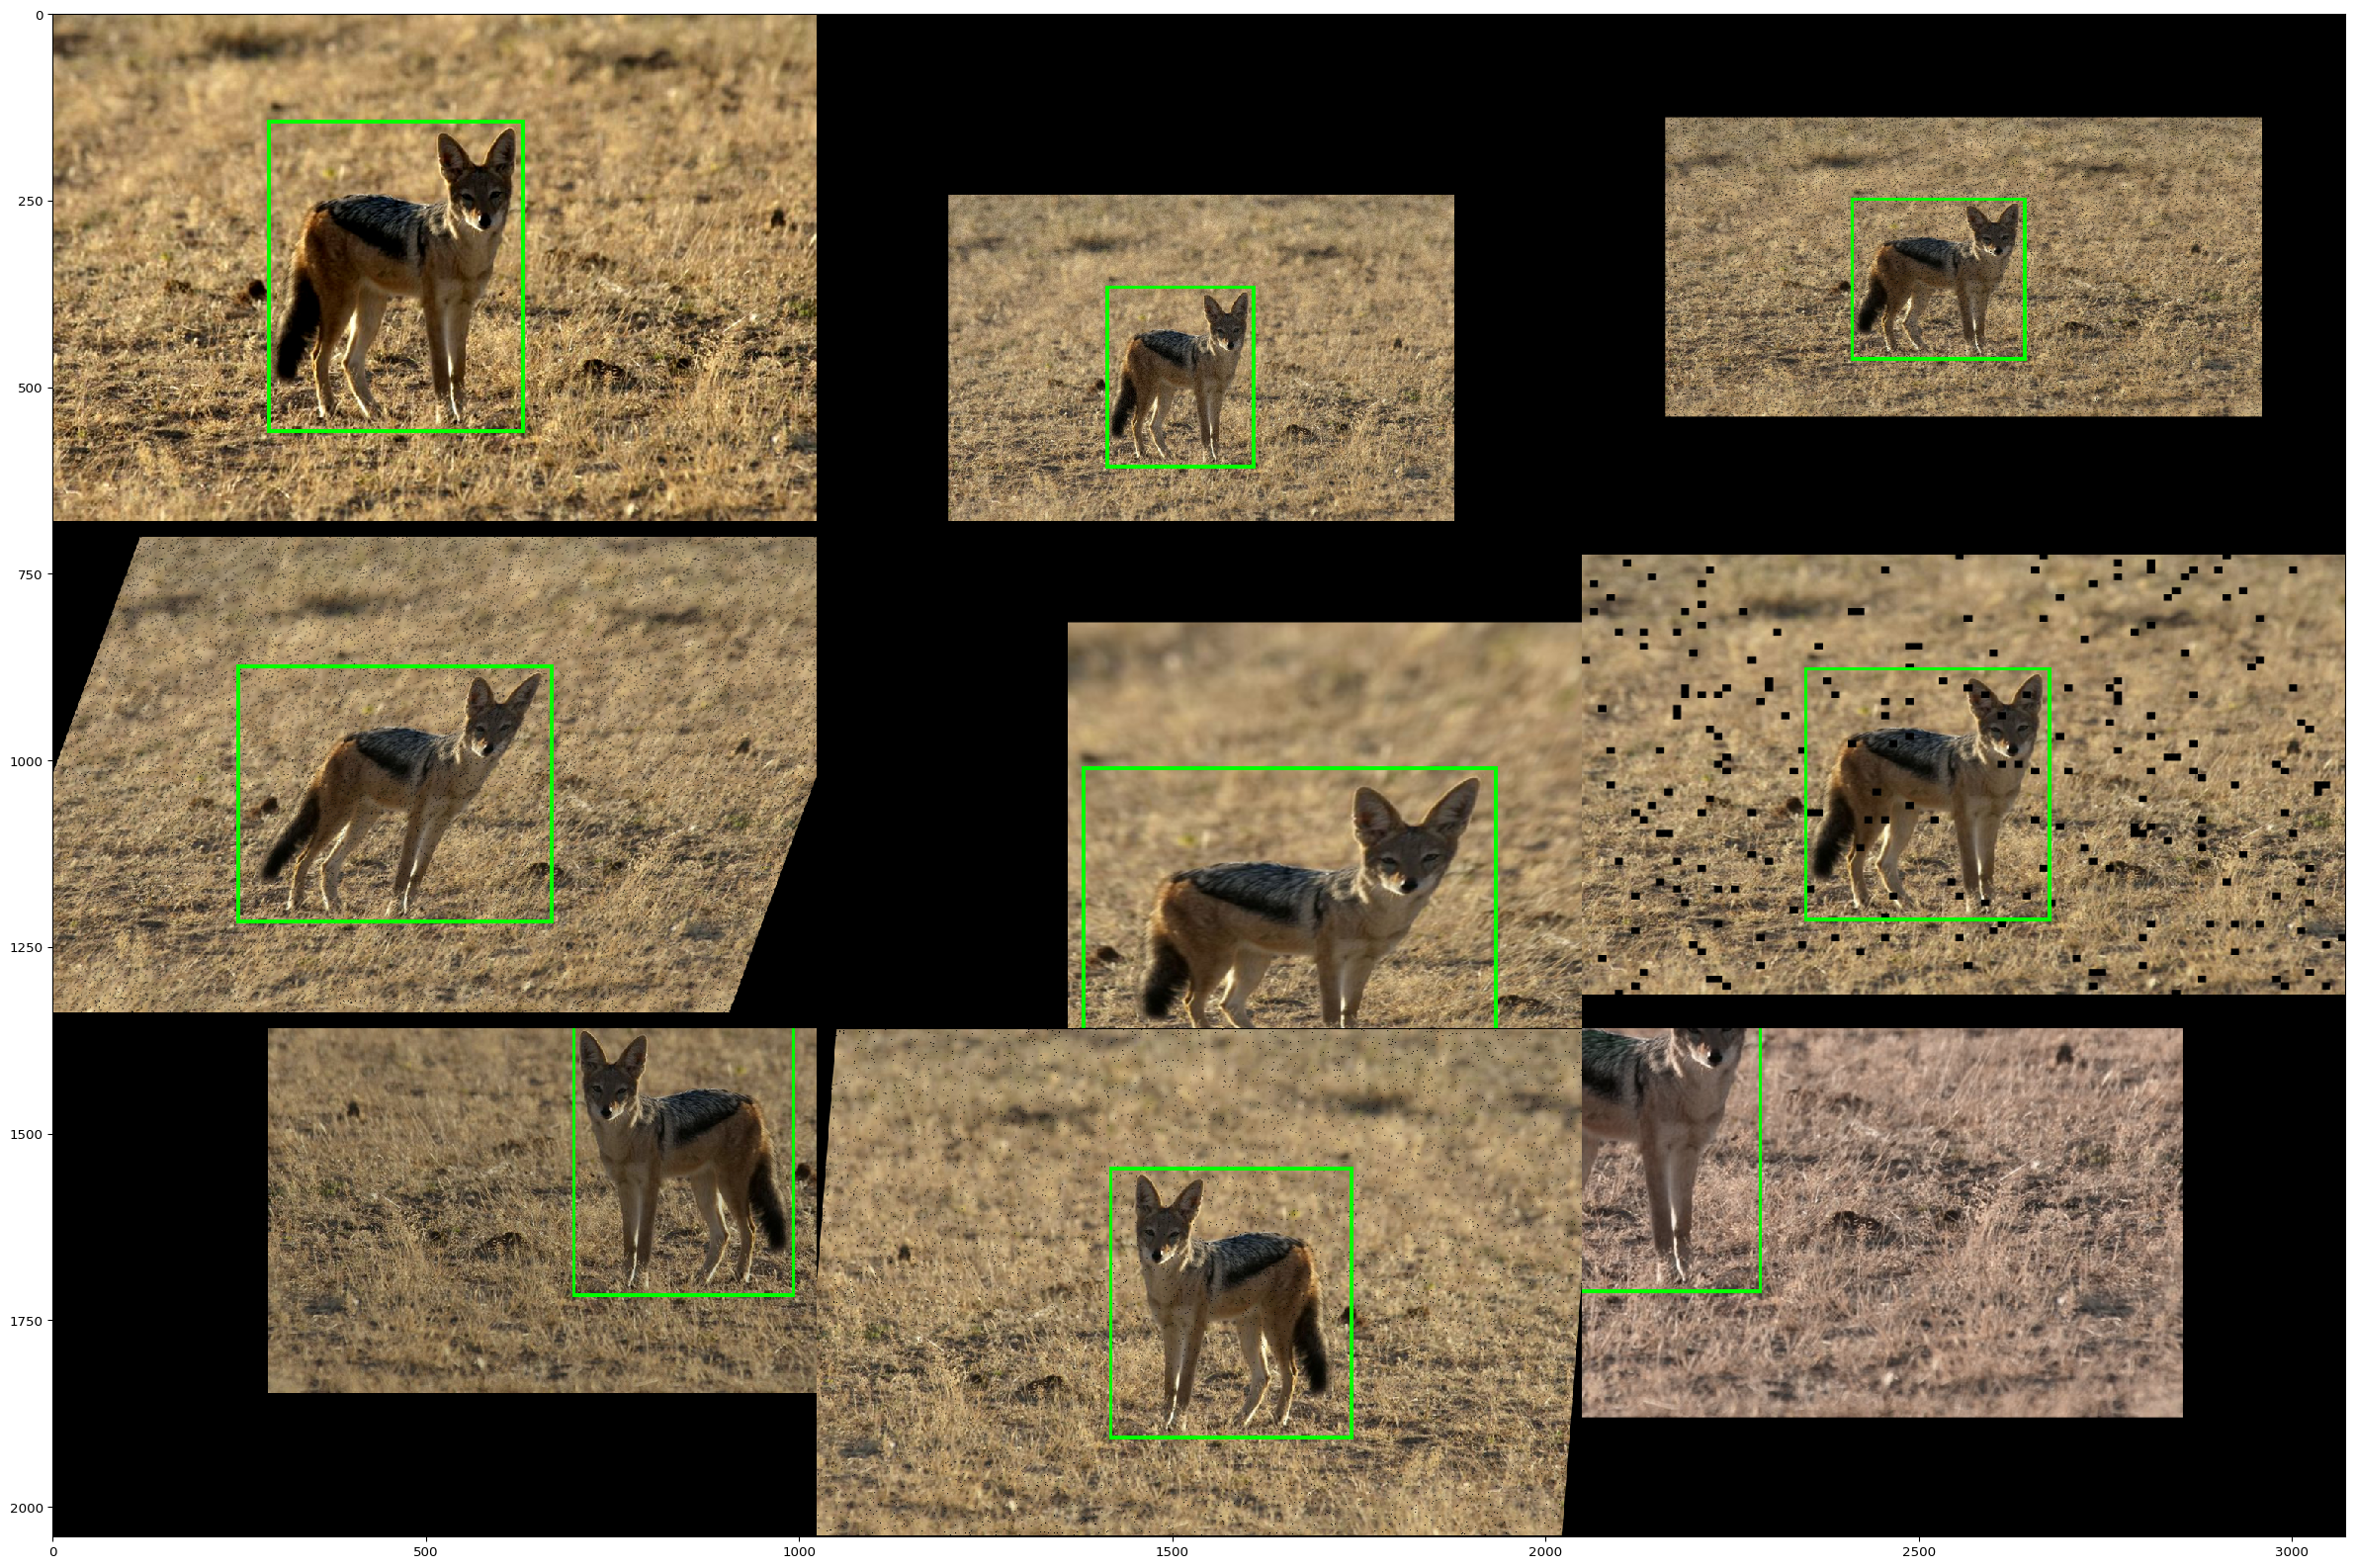
\includegraphics[width=0.8\columnwidth]{Bilder/augmentierung.png}
    \caption{Anwendung von Augmentierungstechniken}
\end{figure}


\section{Training}

Da der Neural Compute Stick mit OpenVino ein eigenes Datei Format 
für die traininerten Modelle verwendet, musste bei der Auswahl
eines Frameworks sowie Models auf die Kompatibilität zu OpenVino 
geachtet werden. 

Verwendete wurde daher das untersstütze Framework Tensorflow, 
um zwei Ansätze zu verfolgen. Der eine verwendet die Api Keras, 
und versucht neben der Klassifikation die Lokalisierung mit 
dieser vorzunahemen, der andere verwendet eine speziell für die 
Objekterkennung konzipierte Api für wie in Abschnitt
 \ref{sec:related_work} beschriebene End-to-End lösungen.

\subsection{Tensorflow Object Detection Api}

Die Tensorflow Object Detection Api ist unter den Research Modellen
\cite{HttpsGithubCom} des offiziellen Tensorflow Repository zu
finden und enthällt implementierungen einiger gängiger Object Detectin
Modelle, wie Single Shot Detectors (SSD) und Faster R-CNNs mit 
verschiedenen Basis CNNs mit vortrainierten Geweichten.

Um die Modelle trainieren zu können, mussten zunächst die 
Trainingsdaten in das binary Dateiformate TFRecords umgewandelt 
werden, welches die Api verwendet. Dieses ist eine Serialisierte 
darstellung der Daten als Protocol Buffer für effiziente Zufriff.



\subsection{Regularisierung}

Um das Overfitting zu vermeiden gibt es wie in \ref{sec:nn} 
beschrieben vershiedene Möglichkeiten.

Untersucht wurde hier

\begin{itemize}
    \item Augmentierung
    \item Early Stopping
    \item \dots weitere zB $L_{1}$, $L_{2}$
\end{itemize}



\subsection{Training grayscale}\label{subsec:train_gray}

Da die Kamera im Infrarot Modus ein Graustufen Bild mit nur einem 
Farbchannel liefert, muss dies für die Inferenz berücksichtigt werden.

Es ergeben sich hier mehrere möglichkeiten:

\begin{enumerate}
    \item Normales (r, g, b) Netz
    \item Ein Farbchannel (gr) Netz
    \item Drei Farbchannel (gr, gr, gr)
\end{enumerate}

Für 1. und 3. Müssen die bilder der Kamera vor der 
Inferenz auf 3 Farbchannel ($3 \times grau$) erweitert werden.
\\
Um das Netz auf einen Channel zu trainieren wurde im config file \dots
\\
Um $3 \times gray$ zu trainieren wurden die Bilder in OpenCV in 
grau convertiert und wieder als jpgs abgespeichert.

Die Ergebnisse sind in Kapitel \ref{kap:eval} dargestellt.


\section{Parameter Optimierung}
einstellungen im Config File\\
tensorflow graph oder plot zeigen\\
loss erklären (mit formel und für train und eval)



% \section[\thesection \  Evaluierung]{Evaluierung}\label{sec:evaluation}

\begin{frame}{Mean Average Precision (mAP)}
    \fontsize{9pt}{9pt}\selectfont
    \begin{columns}[T]
    \column{0.5\columnwidth}
    \textbf{\normalsize Intersection over Union (IoU)}
    \begin{figure}
        \centering
        \includegraphics[width=0.7\textwidth]{Bilder/IoU.png}                    
    \end{figure}
    \begin{itemize}
        \item $\text{IoU} > 0.5 \rightarrow \textbf{True Positive}$
    \end{itemize}
    
    \column{0.5\columnwidth}
    \visible<2->{
    \textbf{Recall:} Trefferquote
    \begin{equation*}
        \frac{\text{True Positives}}{\text{alle Objekte im Bild}}
    \end{equation*}
    \\[0.2cm]
    \textbf{Precision} Genauigkeit 
    \begin{equation*}
        \frac{\text{True Positives}}{\text{alle Predictions}}
    \end{equation*}
    \\[0.2cm]
    \textbf{Average Precision} für eine Klasse
    \begin{equation*}
        AP = \frac{1}{N}\sum Precision(Recall)
    \end{equation*}
    }
    \end{columns}
    \visible<3->{
    \normalsize
    \begin{block}{Loss}
        \begin{itemize}
            \item \textbf{Lokalisierung:} Bounding Box Regression
            \item \textbf{Klassifizierung:} (Logarithmische) Fehlerberechnung
        \end{itemize}
        \vspace{0.3cm}
    \end{block}
    }
    
\end{frame}



\begin{frame}{Auswirkung von Augmentierung}

    \begin{columns}[T]
        \column{0.05\textwidth}
        \vspace{1.5cm}
        Loss\\
        \vspace{3cm}
        mAP\\
        

        \column{0.45\textwidth}
        \centering
        Ohne Augmentierung
        \begin{figure}
            \centering
            \def\svgwidth{0.75\columnwidth}
            \footnotesize
            \input{Bilder/loss_ohne_aug.pdf_tex}
        \end{figure}

        \begin{figure}
            \centering
            \def\svgwidth{0.75\columnwidth}
            \footnotesize
            \input{Bilder/mAP_ohne_aug.pdf_tex}
        \end{figure}
        

        \column{0.45\textwidth}
        \centering
        Mit Augmentierung

        \begin{figure}
            \centering
            \def\svgwidth{0.75\columnwidth}
            \footnotesize
            \input{Bilder/loss_aug.pdf_tex}
        \end{figure}
        \begin{figure}
            \centering
            \def\svgwidth{0.75\columnwidth}
            \footnotesize
            \input{Bilder/mAP_aug.pdf_tex}
        \end{figure}
        
    \end{columns}
\end{frame}



\begin{frame}{Vergleich Modelle: Genauigkeit - Inferenzzeit}
    \begin{columns}
        \column{0.45\columnwidth}
        \textbf{Inferenzzeit}


\begin{table}[]
    \begin{tabular}{|lccc|}
    \hline
    \multirow{2}{*}{\begin{tabular}[c]{@{}l@{}}Archi-\\ tecture\end{tabular}} & \multirow{2}{*}{\begin{tabular}[c]{@{}c@{}}Base\\ CNN\end{tabular}} & \multicolumn{2}{c|}{Infer FPS}                          \\
                                                                              &                                                                     & \multicolumn{1}{l}{Sync.} & \multicolumn{1}{l|}{Async.} \\ \hline
    \multirow{2}{*}{SSD}                                                      & Mobilenet                                                           & 12,6                      & 33,6                        \\
                                                                              & InceptionV2                                                         & 10,7                      & \textbf{28,3}               \\ \hline
    \multirow{2}{*}{\begin{tabular}[c]{@{}l@{}}Faster\\ R-CNN\end{tabular}}   & InceptionV2                                                         & 0,55                      & \textbf{0,72}               \\
                                                                              & ResNet50                                                            & -                         & -                           \\ \hline
    \end{tabular}
    \end{table}
        
        \column{0.1\columnwidth}
        \column{0.45\columnwidth}

        \visible<2->{
        \textbf{Genauigkeit}
        
        \begin{table}[]
            \begin{tabular}{|lll|}
            \hline
            Model                                                                                             & mAP                                                             & Loss                                                             \\ \hline
            \begin{tabular}[c]{@{}l@{}}SSD InceptionV2\\ +Augmentierung\end{tabular}                          & \begin{tabular}[c]{@{}l@{}}0.55\\ 0.6\end{tabular}              & \begin{tabular}[c]{@{}l@{}}4,4\\ 4,1\end{tabular}                \\ \hline
            \begin{tabular}[c]{@{}l@{}}Faster R-CNN\\ +Augmentierung\\ +Dropout\\ +L2 Regularis.\end{tabular} & \begin{tabular}[c]{@{}l@{}}0.67\\ 0.7\\ 0.7\\ adsf\end{tabular} & \begin{tabular}[c]{@{}l@{}}0.82\\ 0,7\\ 0.66\\ adfs\end{tabular} \\ \hline
            \end{tabular}
            \end{table}
        }
    \end{columns}
    
    \visible<3->{
    \begin{itemize}
        \centering
        \item Je genauer, desto langsamer!
    \end{itemize}
    }
    \end{frame}

% %##########################  CHAPER 6: APPLICATION  #######################

\chapter{Entwicklung der Anwendung}\label{kap:application}


Dieses Kapitel beschreibt die Realisierung der
Anwendung, als autonomes Kamerasystem zur
Wildtiererkennung.

Zunächst werden dabei die verwendeten Hardwarekomponenten 
erläutert.

Im zweiten Abschnitt wird die Implementierung der 
Inferenz, für eines der trainierten Modelle, 
sowie einer geeigneten Kommunikationsmöglichkeit 
zur Übertragung der Daten beschrieben.


%-------------------------  SECTION 1: AUFBAU  ------------------------
\section{Hardware}\label{sec:aufbau}


Der Aufbau der Anwendung besteht aus einem, in Abbildung 
\ref{fig:raspberrypi} dargestellten Raspberry Pi 4,
auf dem der Programmcode ausgeführt wird,
sowie dem Neural Compute Stick 2 für die Inferenz,
welcher über eine USB Schnittstelle
mit dem Raspberry Pi verbunden wird.

Zur Aufnahme der Bilder wurde das in 
Abbildung \ref{fig:rpicam} dargestellte 
Raspberry Pi Kamera Modul,
mit einem 5MP OV5647 Sensor der Marke Longrunner
verwendet.
Dieses ermöglicht, durch mechanisches zu und abschalten
eines Infrarot Filters vor die Linse, zwischen Tag- und
Nachtsicht zu wechseln.
Der dafür verwendete Magnetschalter wird automatisch 
über einen Helligkeitsensor getriggert.
Im Infrarotmodus befindet sich der Filter nicht 
vor der Linse, sodass neben den elektromagnetischen 
Wellen des Sichtbaren Lichts, auch die des 
langwelligeren des Infrarot Spektrums (850nm) 
auf die Linse treffen und verarbeitet werden können.

Zudem verfügt die Kamera über zwei Infrarot LEDs, 
sodass auch Aufnahmen, in bis zu 3m Entfernung,
in völliger Dunkelheit gemacht werden können.
Diese haben den Vorteil gegenüber normalen LEDs, 
dass die Tiere von keiner Sichtbaren Lichtquelle 
gestört oder verscheucht werden.

Verbunden wird das Kamera Modul über die CSI 
(Camera Serial Interface) 
Schnittstelle des Raspberry Pi's.

\vspace{1cm}
%https://www.amazon.de/gp/product/B07R4JH2ZV/ref=ppx_yo_dt_b_asin_title_o01_s00?ie=UTF8&psc=1
\begin{minipage}{0.55\textwidth}
    \centering
    \includegraphics[width=0.8\textwidth]
    {./Bilder/raspberrypi_4.png}
    \captionof{figure}{Raspberry Pi 4}
    \label{fig:raspberrypi}
\end{minipage}
\begin{minipage}{0.45\textwidth}
    \centering
    \includegraphics[width=0.8\textwidth]
    {longrunner.jpg}
    \captionof{figure}{Longruner Kamera Modul}
    \label{fig:rpicam}
\end{minipage}
\vspace{1cm}


Desweiteren wurde für eine mobile Internetverbindung 
der \textit{Huawei E3531 SurfStick} und zu Stromversorgnung
eine Powerbank verwendet.



% https://www.amazon.de/gp/product/B00HSZEY34/ref=ppx_yo_dt_b_asin_title_o00_s00?ie=UTF8&psc=1


\section{Software}

Die Implementierung der Applikation für den Raspberry Pi
wurde in Python vorgenommen. 
Dabei sind die Funktionalitäten zur Objekterkennung in
dem Script \textit{detection.py} 
und die, zur Herstellung einer Verbindung
und Senden der Daten, in dem 
\textit{connection.py} Script definiert.


Der Kamera Inputstream ist in einem \textit{main.py} Script 
implementiert, von dem aus auch die in Abbildung 
\ref{fig:class_diagram} 
dargestellten Klassen, welche in \textit{detection.py}
und \textit{connection.py} enthalten sind,
verwendet werden.


\vspace{1cm}
\begin{minipage}{0.75\textwidth}
    \centering
    \underline{detection.py}
\end{minipage}
\begin{minipage}{0.25\textwidth}
    \centering
    \underline{connection.py}
\end{minipage}
\begin{figure}[H]
    \centering
    \newcommand\restoreuscatcode{\catcode`\_=8 }
\tikzset{every picture/.prefix style={execute at begin picture=\restoreuscatcode}}


\begin{tikzpicture}   
    
            \umlclass[x=-0.5, y=0.2]{Motion}{ 
              statick\text{\_}background : np.array
              }{ 
              + detect\text{\_}motion(frame) : bool: \\
              + reset\text{\_}background() : void
            }
        
            \umlclass[y=-4.2]{InferenceModel}{ 
                plugin : ie\text{\_}api.IEPlugin\\
                string : device
                }{ 
                + init(device)\\  
                + create\text{\_}exec\text{\_}infer\text{\_}model(.xml, .bin, NReq)\\: ExecInferModel
              }
        
            \umlclass[y=-1, x=5.6]{ExecInferModel}{ 
                exec\text{\_}net : ie\text{\_}api.ExecutableNetwork\\
                labels : list\\
                input\text{\_}blob : \textit{input\text{\_}shape}\\
                output\text{\_}blob : \textit{output\text{\_}shape}\\
                current\text{\_}frame : dict()\\
                detected\text{\_}objects : dict()

                }{ 
                + init(exec\text{\_}net, labels, input\text{\_}blob)\\
                + infer\text{\_}frames() : \textit{status} \\
                - save(class\text{\_}id) : void
                }
        
    
        \umlclass[x=11.5, y=-2]{Connection}{ 
            loin\text{\_}data : string
            }{ 
            + login(device\text\_name) : bool \\
            + connect() : (server, port)\\
            + send(server, port, file) : bool\\
            + disconnect() : bool\\
            + send\text{\_}email(addr, msg) : bool
          }

    
    \end{tikzpicture}
            
    \caption{Klassendiagramm der Anwendung}
    \label{fig:class_diagram}
\end{figure}
\vspace{1cm}


Die Klasse \textit{Motion} dient zur Erkennung von Bewegungen 
im Kamera Input Stream, \textit{InferenceModel} und
\textit{ExecInferModel} realisieren die Inferenz 
eines trainierten Modells und die Klasse 
\textit{Connection} dient dem Aufbau einer
Verbindung zu einem anderen Gerät, sowie dem Senden
der erkannten Bilder darüber.


Durch geeigneten Implementierung des Applikationsablaufes,
sollte eine Möglichkeit gefunden werden, trotz 
der langsamen Inferenzzeit, mit dem Faster R-CNN
alle relevanten Frames, also die, in denen Tiere zu vermuten
sind, inferieren zu können.
Dafür wurde die Annahme gemacht, dass zur Laufzeit der 
Anwendung, nicht durchgehend inferiert werden muss,
sich also Zeitweise keine Tiere und damit auch keine 
Bewegung vor der Kamera befinden.

Um Bewegungen feststellen zu können, 
wurde, mithilfe der Library \textit{OpenCV}
ein Bewegungsmelder implementiert.
Dieser speichert zu Begin des Kamera Streams ein Referenz
Frame ab, mit dem alle weiteren Frames verglichen werden.
Beträgt der Abstand, der einzelnen Pixelwerte im 
Graustufenbereich mehr, als ein bestimmter 
Threshhold, wird dies als Bewegung gewertet.
Indem nun die Frames, welche der Kamera Stream permanent 
liefert, zunächst auf Bewegung überprüft werden, 
lässt sich unnötiges inferieren vermeiden,
was Zeit und und Energie kostet.
Frames, die Bewegung enthalten, und aufgrund der langsamen 
Inferenzzeit des Faster R-CNN nicht sofort inferiert 
werden können, werden in einem Buffer zwischen 
gespeichert und in Phasen, zu denen keine Bewegung stattfindet, 
inferiert.

Dafür musste der in Abschnitt \ref{sec:infertime} beschriebene
asynchrone Inferenzablauf dahingehend angepasst werden,
dass kein blockierendes warten auf 
ein Inferenzergebnis stattfindet,
wodurch die Inferenz komplet zeitasynchron zu 
den Inputframes abläuft.
Der Gesamtablauf der Applikation ist in Abbildung 
\ref{fig:flowchart_appl} 
schematisch als Flussdiagram dargestellt.

\vspace{1cm}
\begin{figure}[H]
    \centering
    \tikzset{
    desicion/.style={
        diamond,
        draw,
        text width=4em,
        text badly centered,
        inner sep=0pt
    },
    block/.style={
        rectangle,
        draw,
        text width=10em,
        text centered,
        rounded corners
    },
    arrow/.style={
        draw,
        >=latex,
        ->
    }
}


\begin{tikzpicture}
    \node (A) [desicion] {entschei\\dung};
    \node (B) [block, below of=A, node distance=3cm, text width=5em] {bock};
    \node (C) [block, right of=A, node distance=0.5\textwidth] {noch ein\\bock};


    \draw[arrow] (A) --  node [left, fill=white!30] {yes} (B);
    \draw[arrow] (A) -- node [below, near end] {crap} (C); 
    \draw[arrow] (B) -| node [near start, fill=white] {yes} (C);

\end{tikzpicture}
    
    \caption{Schematischer Ablauf des Applikationscode}
    \label{fig:flowchart_appl}
\end{figure}
\vspace{1cm}


Wird in inferierten Frames mehrfach nichts 
erkannt, wird das Referenz Frame des 
Bewegungsmelders durch ein aktuelles Frame ersetzt.

Erkannte Objekt werden in einer
Datenstruktur (Pytho Dictionary) zusammen 
mit Klassenname (cls), Wahrscheinlichkeit(p)
Anzahl an Erkennungen (N) sowie die Bounding 
Box Koordinaten (Roi, (Region of Interest)) 
abgespeichert.

Nach einer bestimmte Anzahl 
an Erkennungen des selben Objekts, wird dieses 
als lokale Bilddatei abgespeichert und ein 
Send-Requst an das Main Script zurückgegeben.

Dieses prüft dann ob eine Verbindung zu einem 
anderen Gerät besteht, stellt diese gegebenenfalls her,
und sendet die lokal abgespeicherten Bilder.

Um nicht permanent die Verbindung zu einem Pc aufrecht erhalten 
zu müssen, was das Datenvolumen des mobilen Internets
schneller aufbrauchen würde, wird diese nach einer 
bestimmte zeit ohne Bewegung getrennt.

Im folgenden werden die Funktionsweise der 
Inferenz sowie der Verbindungsaufbau 
genauer erklärt.


\subsection*{Inferenz}

Der im Abschnitt \ref{sec:infertime} beschriebene asynchronen
Inferenzablauf wurde dahingehend angepasst, dass eine beliebige
Anzahl an Inferenz Requests verwendet werden kann 
und dass das Warten auf ein Inferenz Ergebnis
nicht mehr blockierend ist.
Dafür wurde der Timeout in der Wait-Funktion auf 
$0ms$ gesetzt.
In Algorithmus \ref{code:infer_async_neu} ist 
der Inferenzablauf als Pseudocode dargestellt.

\begin{algorithm}[H]
    \caption{Asynchrone Inferenz, ohne Blockierung}
    \label{code:infer_async_neu}
    \begin{algorithmic}
    \WHILE{\TRUE}
    \STATE capture FRAMES
        \FOR{all InferRequests}
            %\STATE Status $\leftarrow$ \textbf{wait} for 
            % InferRequest
            \IF {\textbf{wait} for InferRequest \textbf{is} 0}
                \STATE Result $\leftarrow$ InferRequest.output
            \ENDIF
            \IF {Buffer \textbf{not} empty}
                \STATE preprocess InferRequest
                \STATE \textbf{start} InferRequest
            \ENDIF
            \IF{Result not NULL}
                \STATE process Result
            \ENDIF
        \ENDFOR
    \ENDWHILE
    \end{algorithmic}
\end{algorithm}    





\subsection*{Connection}

Um die Bilder mit erkannten Tieren an ein anderes Gerät 
z.B. einen Pc senden zu können, musste eine Verbindung
hergestellt werden, die auch über verschiedene Netzwerke 
hinweg funktioniert.

Um unabhängig von Router Konfigurationen und Firewall 
Einstellungen zu sein, wurde mithilfe des
Dienstes \textit{remot3.it} \cite{remoteit}
eine Cloudbasierte Remote Verbindung hergestellt.

Mit dieser war es möglich eine Remote Proxy SSH Verbindung, 
über das Internet zu einem anderen Gerät herzustellen.

\begin{figure}[H]
    \centering
    \def\svgwidth{0.7\textwidth}
    \input{Bilder/diagram-connect.pdf_tex}
    \caption{Prinzip Proxy Verbindung}
    \label{fig:remoteit}
\end{figure}

Da die Daten vom Raspberry Pi aus automatisiert gesendet 
werden sollen, wurde der Pc, an den 
sie Daten gesendet werden, als Remote Gerät implementiert.

Gesendet wurden die Daten über das \textit{Secure Copy Protocol},
welches das hergestellte \textit{Secure Shell Protocol (SSH)}
verwendet.
Dieses lässt sich über folgendes Kommando,
welches im \textit{connection.py}
Script ausgeführt wird, bedienen:
\begin{itemize}
    \item[\texttt{\$}] \texttt{scp -P port file.jpg 
    user@proxyadresse /zielpfad/file.jpg}
\end{itemize}

Server und Port werden dabei von remote.it
generiert, \textit{file.jpg} ist das zu sendende Bild und
\textit{user} der Nutzername des Geräts,
an welches gesendet wird.
Um das Einloggen sowie den Verbindungs Auf- und Abbau 
über remote.it zu einem Gerät automatisieren zu können,
bietet remote.it eine API mit der über Post- und Get Requests
die Befehle dafür programmatisch aufgerufen werden können.

Um den Nutzer bei einer Erkennung automatisch 
per Email zu benachrichtigen, wurde 
eine Funktion implementiert, welche das 
\textit{Smart Mail Transfer Protpkol (SMTP)} 
verwendet.

% \chapter{Test und Validierung}\label{kap:testvalidierung}


% \chapter{Zusammenfassung}\label{kap:zusammenfassungausblick}


Ziel der Arbeit war es, ein autonomes
Kamerasystem zur Wildtierkennung
mithilfe Neuronaler Netze zu entwickeln.
Dafür wurden vortrainierte, \Gls{cnn}-basierte, 
Deep-Learning-Modelle zur Objekterkennung
auf einen geeigneten Datensatz trainiert.
Dadurch sollte es möglich sein, nicht 
nur die Anwesenheit eines Tieres 
zu erkennen, sondern auch eine 
Klassifizierung der Tierart 
vorzunehmen. Auf diese Weise kann das System 
gezielter für eine bestimmte
Anwendung eingesetzt werden.
Zur Realisierung wurde neben einem \textit{Raspberry
Pi} sowie einer nachtsichtgeeigneten 
Kamera der \textit{Neural Compute Stick 2}
von \textit{Intel} verwendet, um die 
Verarbeitung der Daten auf dem 
Gerät ausführen zu können.
\vspace{0.5cm}


Für das Training wurde ein Datensatz, 
bestehend aus 9 Wildtierklassen verwendet,
welcher aus \textit{Open Images} heruntergeladen werden konnte.
Anschließend wurden die Daten 
für das Training aufbereitet und
zur Evaluierung in verschiedene 
Sets aufgeteilt.
Das Training wurde dann mithilfe des 
\Glspl{framework} \textit{TensorFlow} durchgeführt,
wobei die Modelle Single Shot Detector (SSD) und
Faster R-CNN mit verschiedenen
Basis-\Glspl{cnn} und Parametereinstellungen
verwendet wurden.
Durch anschließende Evaluierung konnte 
festgestellt werden, welches Modell sich,
bezogen auf Genauigkeit und Geschwindigkeit,
am besten für die Anwendung eignet.
Der letzte Schritt war die Inferenz zusammen 
mit dem Anwendungscode für den \textit{Raspberry Pi} 
zu implementieren, wofür mit \textit{OpenVino} gearbeitet 
wurde.
\vspace{0.5cm}

Die Evaluierung der trainierten Modelle zeigte,
dass eine erhöhte Genauigkeit mit einer 
langsameren Inferenzzeit einhergeht.
Durch umfangreiche Testläufe mit 
variierenden Parametern konnten die 
optimalen Konfigurationen für die Anwendung 
erforscht und somit die Ergebnisse verbessert 
werden.

Daraus resultierend wurde für die Anwendung das 
Faster R-CNN Modell mit InceptionV2 
als Basis-\Gls{cnn} gewählt. Dieses erreichte 
durch ein Training von 500k Iterationen 
auf den \textit{Open Images} Datensatz 
einen mAP-Wert von 0.7 und einen Loss-Wert von 0.74.
Der Datensatz wurde durch geometrische und 
pixelwertbezogene Veränderungen der Bilder 
augmentiert, wodurch für jede Klasse 3000 
Bilder für das Training vorhanden waren.

Durch einen asynchronen Inferenzablauf 
mit drei Inferenz-Requests konnte die 
Inferenzzeit für das Faster R-CNN 
von 0,63 \Gls{fps} auf 0,75 \Gls{fps} 
erhöht werden. 
Indem ein Bewegungsmelder sowie ein 
Zwischenspeichern der Frames im 
Anwendungsablauf implementiert wurde, ließ sich 
die Performance weiter verbessern.


\newpage

\bibliography{Bachelor_Arbeit,Bilder,weitere}
\bibliographystyle{ieeetr}

\appendix

\chapter{Beispiel für ein Kaptel im Anhang}\label{appkap:bsp1}

\section{Bsp für ein Abschnitt im Anhang}\label{appsec:bsp2}

\end{document}

